\usetikzlibrary{arrows.meta,calc}
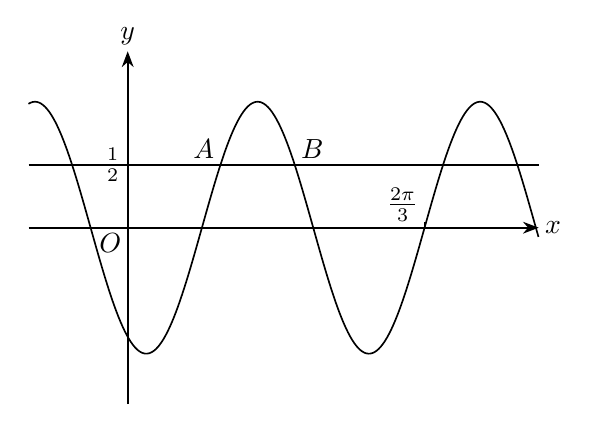
\begin{tikzpicture}[x=1.8cm,y=1.6cm,line width=.6pt,>=Stealth,font=\normalsize]
% axes beyond last ticks (x to 2.9 > 2pi/3, y to +-1.4)
\draw[->] (-0.7,0)--(2.9,0) node[right,inner sep=0pt,xshift=2pt] {$x$};
\draw[->] (0,-1.4)--(0,1.4) node[above,inner sep=0pt,yshift=2pt] {$y$};
\node[below left,inner sep=0pt,xshift=-2pt,yshift=-2pt] at (0,0) {$O$};
% ticks
\draw[line width=.6pt] (2.0943951,0)--(2.0943951,0.045);
\node[above left,inner sep=0pt,xshift=-2pt,yshift=2pt] at (2.0943951,0) {$\frac{2\pi}{3}$};
\draw[line width=.6pt] (0,0.5)--(0.04,0.5);
\node[left,inner sep=0pt,xshift=-2pt] at (0,0.5) {$\frac12$};
% exact sine f(x)=sin(4x-8pi/3) via degrees: sin(4*deg(x)-480)
\draw[domain=-0.7:2.9,samples=250] plot (\x,{sin(4*deg(\x)-480)});
% horizontal y=1/2
\draw (-0.7,0.5)--(2.9,0.5);
% A rising (5pi/24), B falling (3pi/8) below line with 2pt gap
\node[above left,inner sep=0pt,xshift=-2pt,yshift=2pt] at (0.65449847,0.5) {$A$};
\node[above right,inner sep=0pt,xshift=2pt,yshift=2pt] at (1.17809725,0.5) {$B$};
\end{tikzpicture}
